\subsection{图卷积神经网络}
卷积神经网络(CNN)无法处理非欧几里得(Non Euclidean Structure)的数据,即传统的离散卷积在Non Euclidean Structure的数据上无法保持平移不变性。因为在拓扑图中每个顶点的相邻顶点数目都可能不同,那么也就无法用一个同样的尺寸的卷积核来进行卷积运算。CNN无法处理Non Euclidean Structure的数据,又希望在拓扑图上有效的提取空间特征来进行学习,所以GCN成为研究重点。

卷积图神经网络(ConvGNN)与循环图神经网络(RecGNN)密切相关。ConvGNN不是使用收缩约束来迭代节点状态,而是在结构上使用固定数量的层(在每一层中具有不同的权重)来解决循环的相互依赖性。图\ref{fig:RGNN_CGNN}说明了这一主要区别。由于图卷积更加有效且易于与其他神经网络进行结合,因此,ConvGNN近年来得到了迅速的发展。ConvGNN分为两类,基于频谱的ConvGNN和基于空间的ConvGNN。基于频谱的ConvGNN通过从图信号处理的角度引入滤波器来定义图卷积,其中图卷积运算被解释为消除图信号中的噪声。基于空间的ConvGNN通过信息聚合,以定义图卷积。自从GCN弥合了基于频谱的方法与基于空间的方法之间的差距以来,基于空间的方法由于其引人注目的效率,灵活性和通用性而迅速发展。

\begin{figure}[htbp]
	\centering 
	\subfigure[循环图神经网络(RecGNNs)。 RecGNN在更新节点表示中使用相同的图复现层(Grec)。]
	{
		\begin{minipage}[t]{0.5\textwidth}
			\centering         
			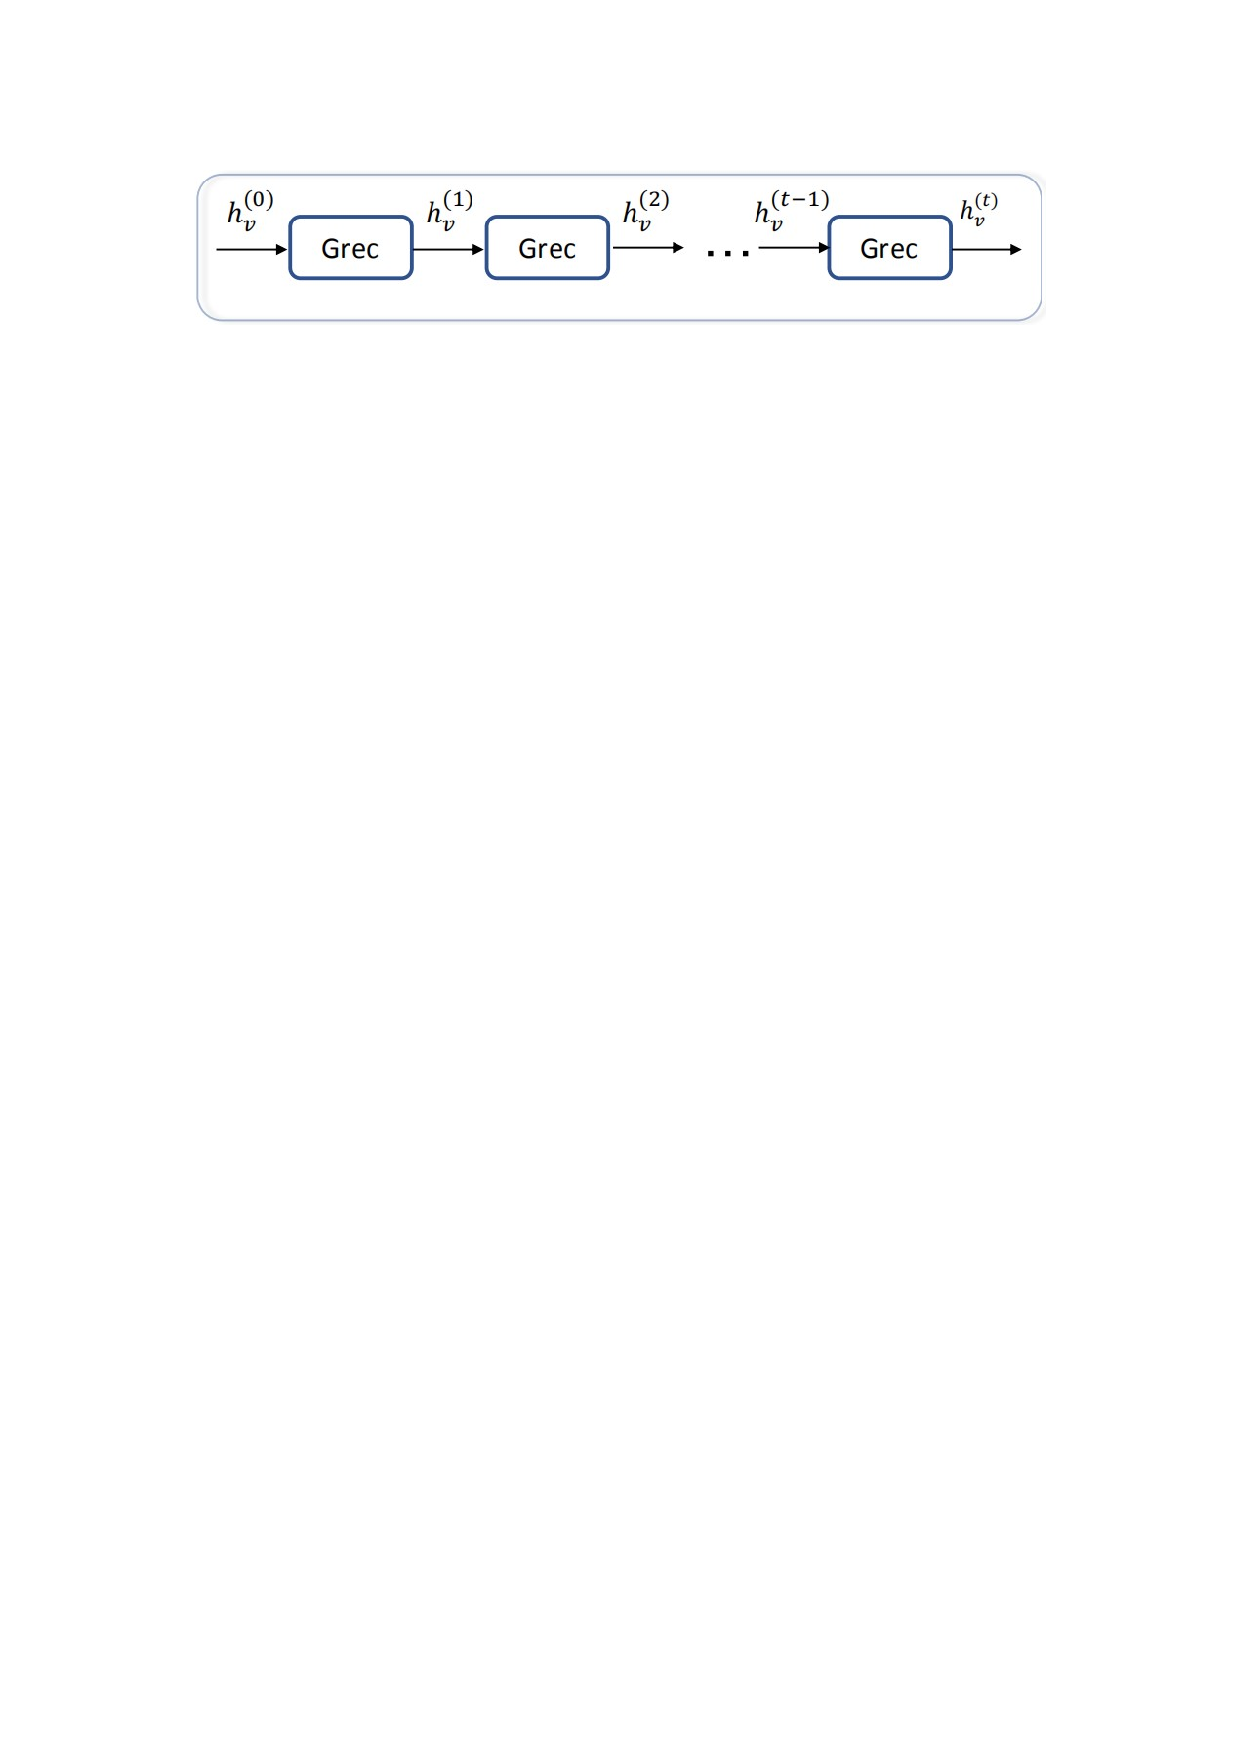
\includegraphics[width=1\textwidth]{Fig/RecGNNa.pdf}   
		\end{minipage}
	}

	\subfigure[卷积图神经网络(ConvGNN)。ConvGNN在更新节点表示时使用不同的图卷积层(Gconv)] 
	{
		\begin{minipage}[t]{0.5\textwidth}
			\centering      
			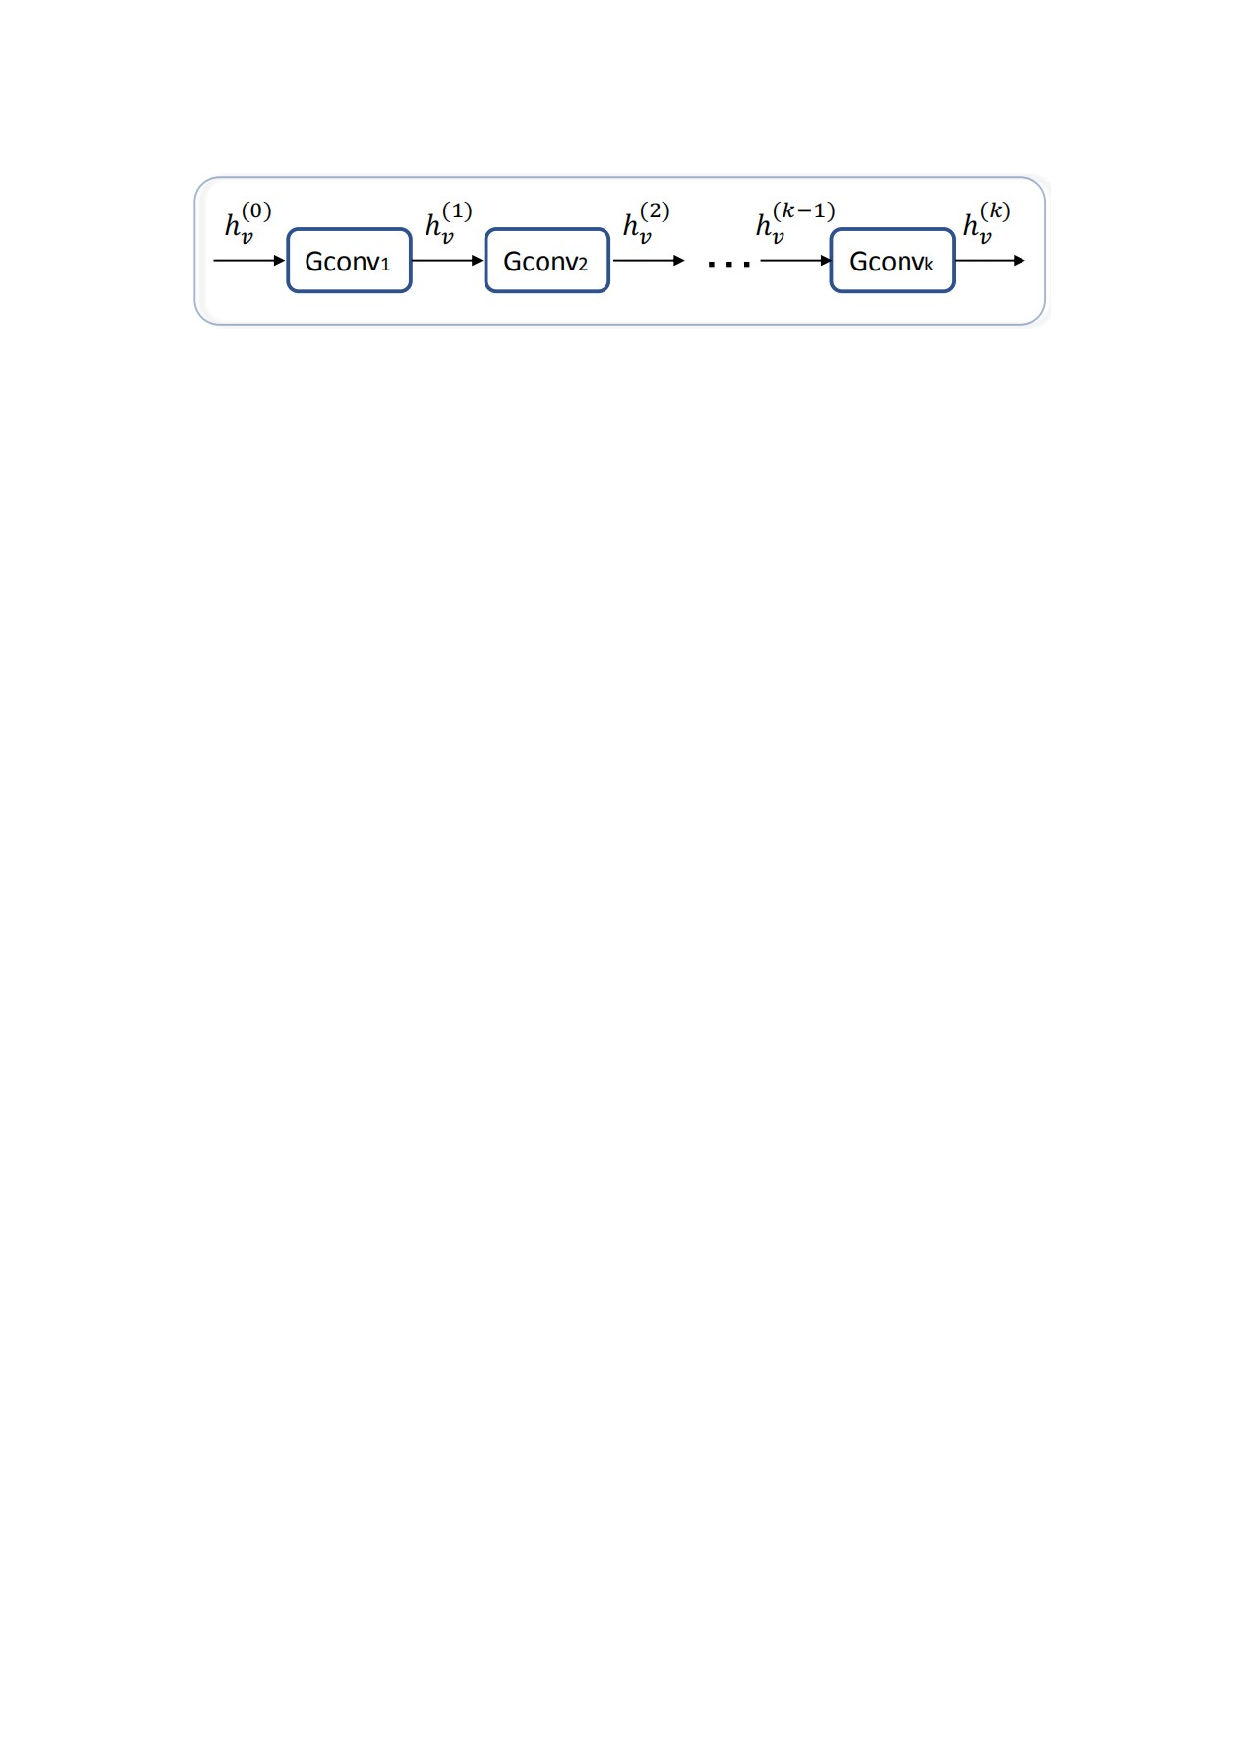
\includegraphics[width=1\textwidth]{Fig/CGNNb.pdf}   
		\end{minipage}
		
	}
	\caption{RecGNNs and ConvGNNs}
	\label{fig:RGNN_CGNN} 
\end{figure}	

\subsubsection{基于频谱的ConvGNNs}

基于频谱的方法在图形信号处理中具有坚实的数学基础,一般假设是无向图。无向图的数学表示是归一化图拉普拉斯矩阵,定义为
\[L=I_n-D^{-\frac{1}{2}}AD^{-\frac{1}{2}}\]
其中,$D$是节点的对角矩阵。归一化图拉普拉斯矩阵具有实对称半正定的性质。利用该属性,归一化的拉普拉斯矩阵可以被分解为
\[L=U\sum U^T\]
输入信号$x$和滤波器$g\in R^N$的图形卷积定义为
\[
x*_Gg=\mathcal{F}^{-1}(\mathcal{F}(x)\bigodot \mathcal{F}(g))
\]
其中,$\bigodot$表示Hadamard矩阵乘积。如果,$g_{\theta}=diag(U^Tg)$,卷积就会简化为
\[
x*_Gg_{\theta}=Ug_{\theta}U^Tx
\]
基于频谱的ConvGNNs都遵循这个定义。

频谱卷积神经网络,假设滤波器是一组可学习的参数,并考虑了具有多个通道的图形信号。首先,对图的任何扰动都会导致本征基的变化。其次,学习的过滤器是域相关的,这意味着它们不能应用于具有不同结构的图。第三,特征分解需要$O(n^3)$复杂度。在后续工作中,ChebNet和GCN通过进行一些近似和简化将计算复杂度降低到$O(n)$。

Chebyshev谱CNN(ChebNet)通过特征值对角矩阵的Chebyshev多项式逼近滤波器$g_{\theta}$,学习的权重可以在图表中的不同位置共享。ChebNet的频谱线性映射到[-1,1]。

CayleyNet进一步应用Cayley多项式,它是参数有理复合函数,用于捕获窄频带。CayleyNet的频谱图卷积定义为
\[
x*_Gg_{\theta}=c_0x+2Re\{\sum_{j=1}^{r}c_j(hL-iI)^j(hL+iI)^{-j}x)\}
\]
其中,$Re$返回复数的实部,$c_0$是一个实数系数,$c_j$是一个复数系数,$i$是虚数,$h$是控制Cayley滤波器频谱的参数。在保留空间局部性的同时,CayleyNet显示ChebNet可以被视为CayleyNet的特例。

  
最近的几项工作通过探索替代对称矩阵对GCN进行了改进。自适应图形卷积网络(AGCN)学习由图形邻接矩阵未指定的隐藏结构关系。它通过可学习的距离函数构造所谓的残差图邻接矩阵,该函数将两个节点的特征作为输入。

\subsubsection{基于空间的ConvGNNs}
由于传统CNN在图像上的卷积运算,基于空间的方法是根据节点的空间关系来定义图形卷积。
图像可以被视为图形的特殊形式,每个像素代表一个节点,每个像素直接连接到其附近的像素,如\ref{fig:2DConvs_GConvs}(a)所示。
使用$3\times 3$窗口,每个节点的邻域是其周围的八个像素。
然后通过获取每个通道上的中心节点及其邻居的像素值的加权平均值,将滤波器应用于该区域。
类似地,基于空间的图卷积将中心节点的表示与其邻居的表示进行卷积,以导出中心节点的更新表示,如图\ref{fig:2DConvs_GConvs}(b)所示。从另一个角度来看,基于空间的ConvGNN与RecGNN共享信息传播/消息传递是相同概念。空间图卷积运算实质上沿边传播节点信息。

\begin{figure}[htbp]
	\centering 
	\subfigure[2维卷积]
	{
		\begin{minipage}[t]{0.45\linewidth}
			\centering         
			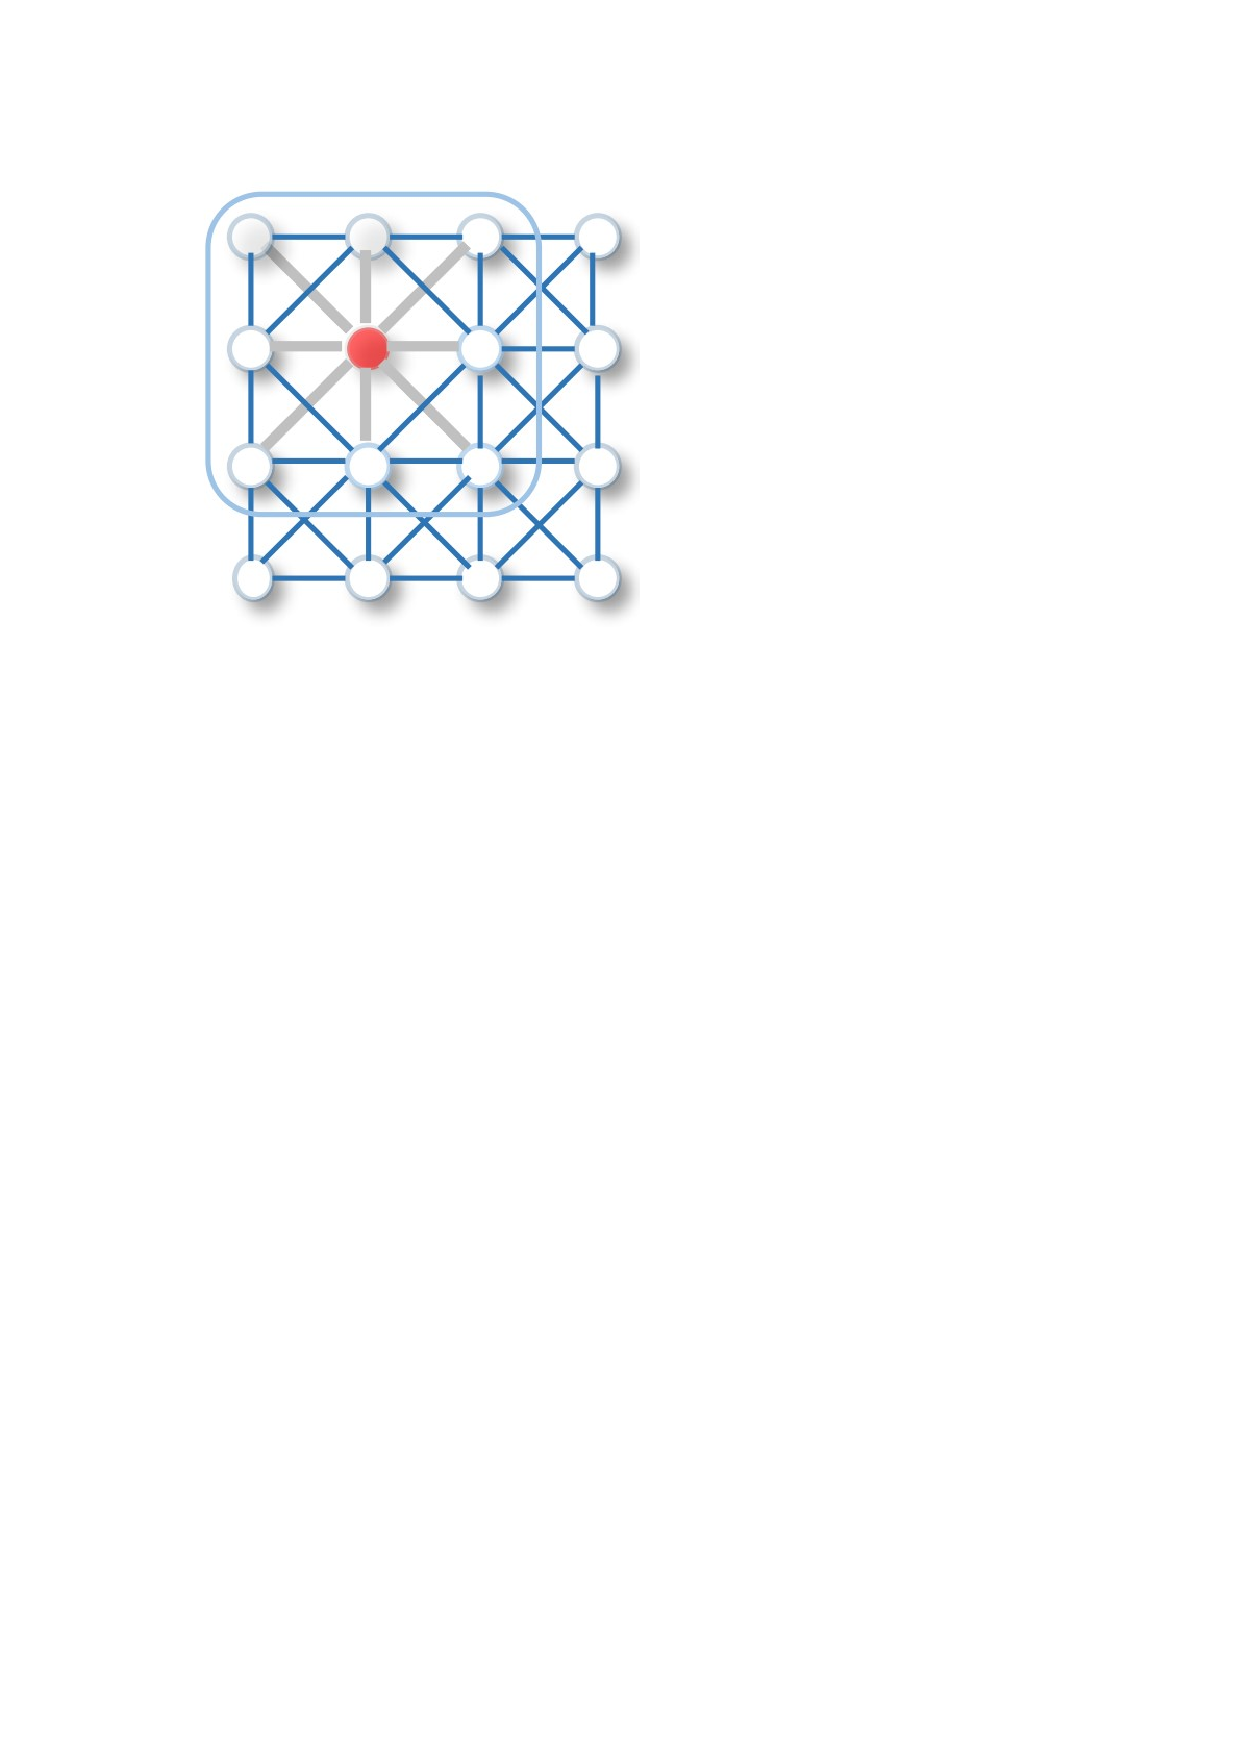
\includegraphics[width=0.5\textwidth]{Fig/2DConv.pdf}   
		\end{minipage}
	}
	\subfigure[图卷积] 
	{
		\begin{minipage}[t]{0.45\linewidth}
			\centering    
			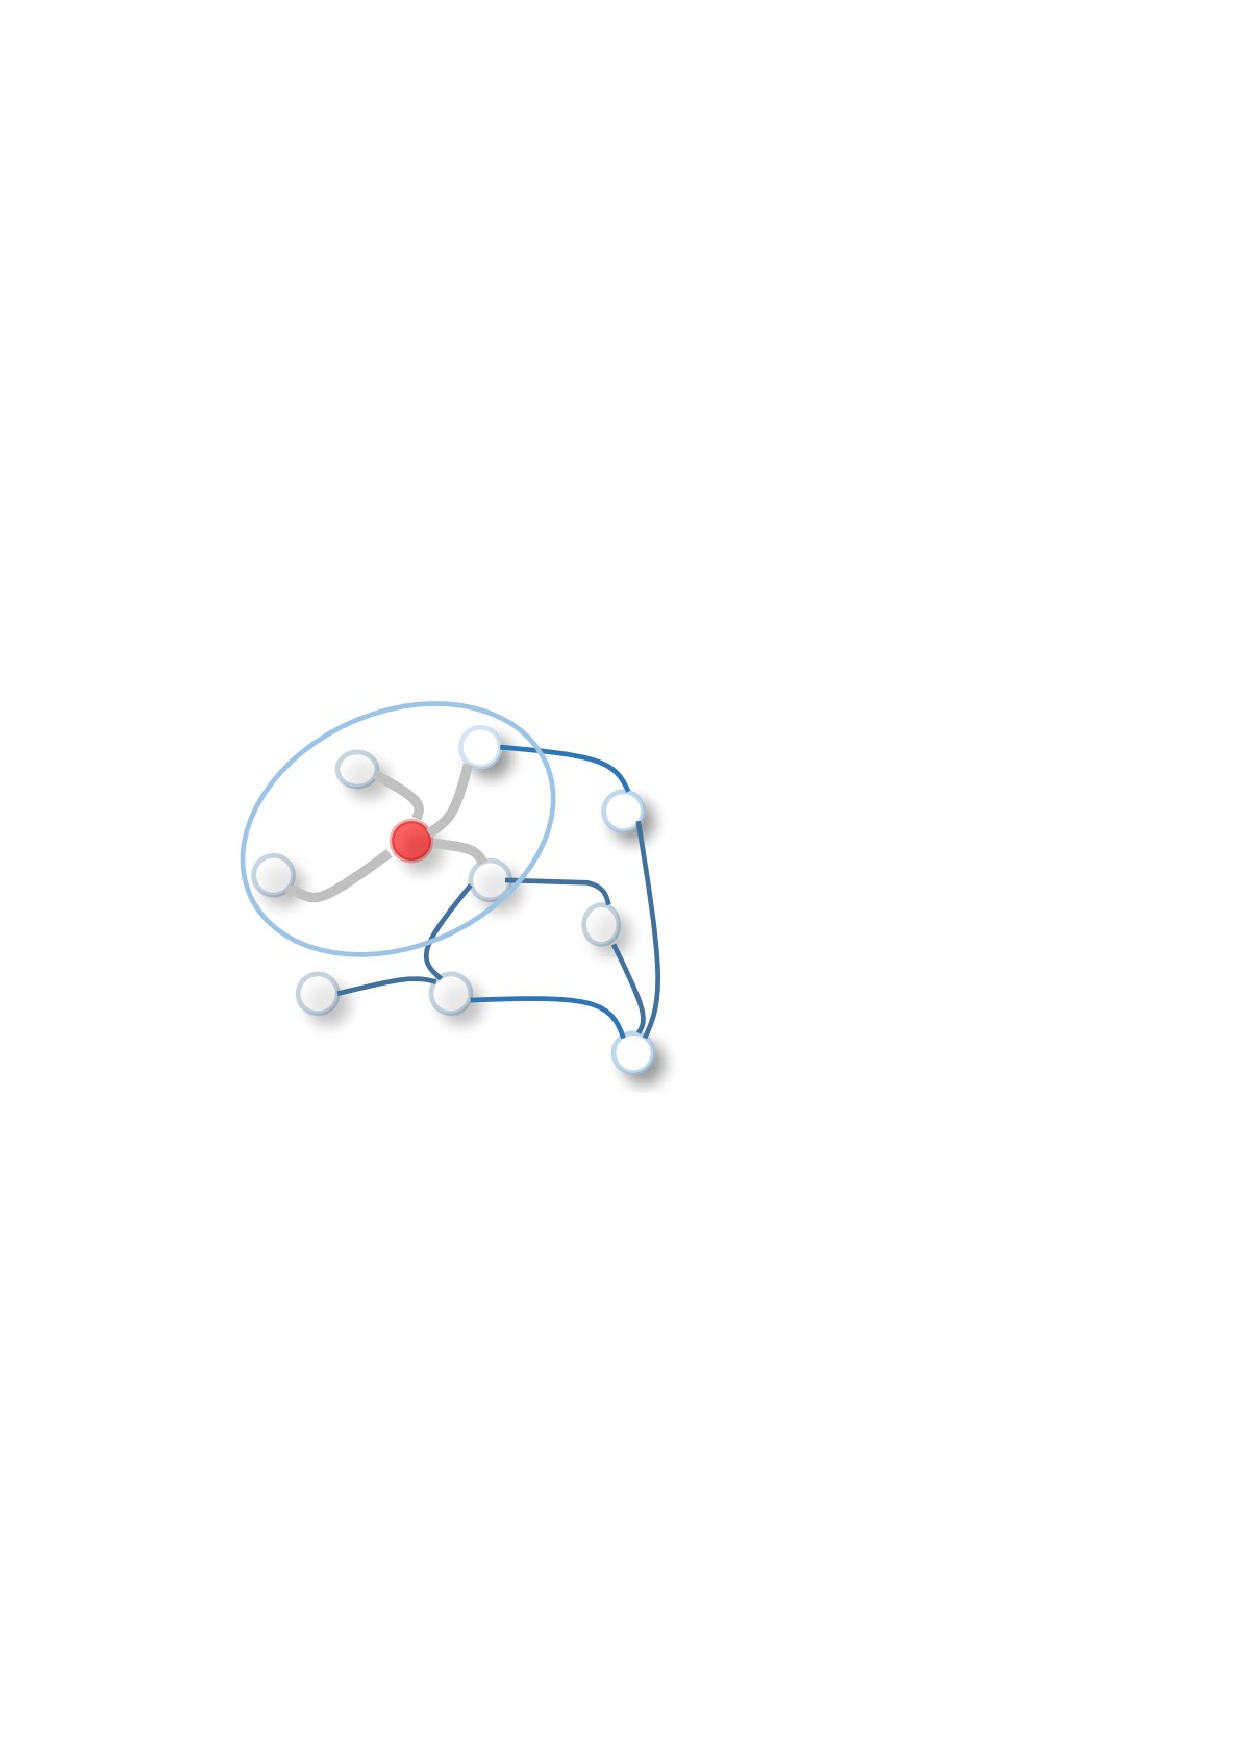
\includegraphics[width=0.5\textwidth]{Fig/GConv.pdf}   
		\end{minipage}
	}
	\caption{2D卷积和图卷积} %  %大图名称
	\label{fig:2DConvs_GConvs}  %图片引用标记
\end{figure}	

图形神经网络(NN4G)是基于空间的ConvGNN的第一项工作。NN4G通过直接汇总节点的邻域信息来执行图卷积。它还会应用剩余连接和跳过连接以存储每个层上的信息。结果,NN4G通过以下方式导出其下一层节点状态 
\[
h_v^{(k)}=f(x_vW^{(k-1)}+\sum_{k-1}^{i=1}\sum_{u\in N(v)}h_u^{(k-1)}\theta^{(k-1)})
\]
其中,$f$是激活函数,初始$h_v^{(0)}=0$

它类似于GCN的形式。主要区别在于NN4G使用非标准化邻接矩阵,这可能会导致数值不稳定性问题。语境图马尔可夫模型(CGMM)提出了一种基于NN4G的概率模型。在保持空间局部性的同时,CGMM具有概率可解释性的好处。

消息传递神经网络(MPNN)概述了基于空间的ConvGNN的一般框架。它将图形卷积视为消息传递过程,其中信息可以直接沿着边缘从一个节点传递到另一个节点。MPNN运行K步消息传递迭代以使信息进一步传播。信息传递函数,即空间图卷积定义如下,

\[
h_v^{(k)}=U_k(h_v^{k-1},\sum_{u\in N(v)}M_k(h_v^{(k-1)},h_u^{(k-1)},x_{uv}^e))
\]
其中 $h_v^0=x_v,U_k,M_k$是通过学习得到的。
由于节点的邻居数量可以从一千到甚至更多,因此无法获取节点邻域的全部大小。GraphSage采用抽样来获得每个节点固定数量的邻居。

图注意力网络(GAT)假设相邻节点对中心节点的贡献既不像GraphSage 那样相同,也不像GCN那样预先确定。GAT采用注意机制来学习两个连接节点之间的相对权重。GAT的图卷积操作定义为,
\[
h_v^{(k)}=\delta(\sum_{u\in \mathcal{N(v)}\cup v}\alpha_{vu}W_k^{(k-1)},h_u^{(k-1)})
\]
其中,$h_v^0=x_v$,注意力权重$\alpha_{uv}$控制节点$u$到$v$的连接权重。计算方法如下,
\[
\alpha_{uv} = softmax(g(a^T[W^{(k-1)}h_v||W^{(k-1)}h_u]))
\]
其中,$g$是一个LeakRELU激活函数,$a$是一个可以学到的参数向量。softmax函数保证了在$v$所有的邻居节点的注意力权重总和到1。

虽然GAT假设注意力头的贡献相等,但门控注意网络(GAAN)引入了一种自我关注机制,该机制计算每个注意力头的额外注意力得分。除了在空间上应用图注意外,GeniePath进一步提出了一种类似LSTM的门控机制来控制图卷积层的信息流。

训练效率方面的改进通常需要训练ConvGNN将整个图形数据和所有节点中间状态保存到内存中。ConvGNN的全批次训练算法明显受到内存溢出问题的困扰,尤其是当一个图包含数百万个节点时。为了节省内存,GraphSage提出了一种针对ConvGNN的批量训练算法。它通过以固定的样本大小按K步递归扩展根节点的邻域来对植根于每个节点的树进行采样。对于每棵采样树,GraphSage通过从下到上分层汇总隐藏节点表示来计算根节点的隐藏表示。

基于频谱和空间模型之间的比较:频谱模型在图形信号处理中具有理论基础。通过设计新的图形信号滤波器,理论上可以构建新的ConvGNN。但是,由于效率,通用性和灵活性问题,与频谱模型相比,空间模型更为可取。首先,频谱模型的效率不如空间模型。频谱模型要么需要执行特征向量计算,要么需要同时处理整个图形。空间模型对大型图更具可伸缩性,因为它们通过信息聚合在图域中直接执行卷积。可以在一批节点而不是整个图中执行计算。其次,依赖于图傅立叶基础的频谱模型不能很好地推广到新图。他们假设一个固定的图。对图的任何扰动都会导致本征基的变化。另一方面,基于空间的模型在每个权重可以在其上的节点上本地执行图卷积,在不同的位置和结构之间轻松共享。第三,基于频谱的模型仅限于在无向图上运行。基于空间的模型更灵活地处理多源图输入,例如边输入,有向图,有符号图和异构图,因为这些图输入可以轻松地合并到聚合函数中。


\subsubsection{图池化模型}
  在GNN生成节点功能之后,我们可以将它们用于最终任务。但是直接使用所有这些特征在计算上具有挑战性,因此需要采用下采样策略。根据目标及其在网络中扮演的角色,该策略给出了不同的名称:(1)池化操作旨在通过对节点进行下采样来减小参数的大小,以生成更小的表示,从而避免排列不变性和计算复杂性问题; (2)读出操作主要用于基于节点表示生成图级表示。他们的机制非常相似。在本章中,我们使用池化来指代应用于GNN的各种下采样策略。

在一些较早的工作中,图粗化算法使用特征分解来基于图的拓扑结构来粗化图。但是,这些方法存在时间复杂性问题。Graclus算法是特征分解的替代方法,用于计算原始图的聚类版本。最近的一些工作将其作为池操作来粗化图。

如今,平均值/最大值/总和池是实现下采样的最原始有效的方法,因为计算池化窗口中的均值/最大值/总和值很快:
\[
h_G=mean/max/sum(h_1^{k},h_2^{k},...,h_n^{k})
\]
其中K是最后一个图卷积层的索引。Henaff等人的研究\cite{henaff2015deep}表明,在网络开始时执行简单的最大/均值池对于降低图域中的维数并降低图傅里叶变换操作的成本尤为重要。

总体而言,池化是减少图形大小的基本操作。然而如何提高汇集的有效性和计算复杂性仍然是一个悬而未决的问题。